
\chapter{System Architecture}  

\section{System Overview}

\section{Fine-tuning}

The Large Language Models (LLM) used for this paper are pre-trained, meaning that the model learned how words relate to each other, the model is trained to understand a language. This process is computationally expensive and requires a large amount of data. Instead of creating a model from scratch, we can teach an existing model to learn a new task such as text classification, translation, generation, or other. This is called fine-tuning, and in this case, it was used to teach the model to classify two types of texts: health-related and misinformation-related. 
\newline
\newline
The health-related dataset comprises over 12,441 tweets extracted from the previous THS project. Said dataset was classified into three categories: related, unrelated, and ambiguous tweets. A second dataset, with 8,762 texts, was created with data from different sources such as news, social media, and blogs classified as misinformation and non-misinformation \textbf{\textit{[Insert References]}}. 

The models used for the classification process were Bert, T5, and LLaMa-2. 

\subsection{Health-Related Classification}


\subsection{Misinformation Classification}


2. Misinformation classification

LR, Batch size, seed, and epochs are static.

- Each model was fine-tune twice.

    1. Sequence classification: 1, 2, or 3; 1 or 2.

    2. Classification with text generation: Related, Unrelated, or Ambiguous; Misinformation or Not Misinformation.

- Weighted average added for the sequence classification.


\section{Paper ETL Pipeline}

\begin{figure}[H]
	\begin{center}
		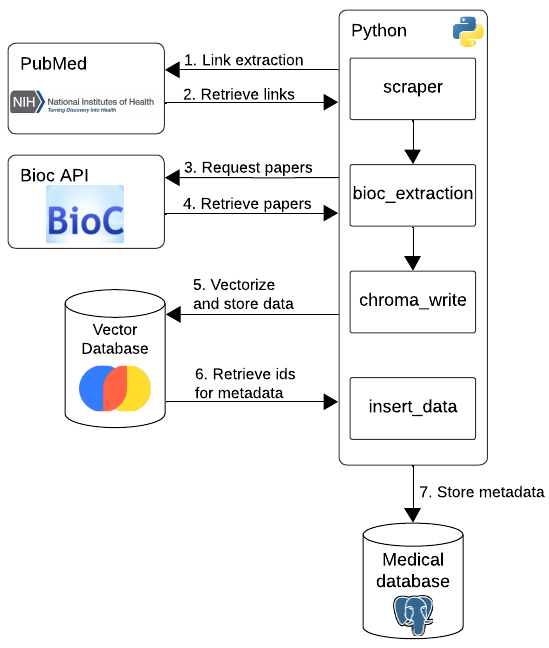
\includegraphics[width=0.75\textwidth]{images/ETL_Pipeline} %specify width
	\end{center}
	\caption{Medical Data Extraction Pipeline} %specify caption
	\label{fig:etl}
\end{figure}

For our models to be able to rebut the misinformation, it needs to use credible sources. We identified PubMed \textbf{[REFERENCES]} to extract the papers and stored them in a vector database.
To extract these papers, we used the BioC API \cite{bioinformatics} that contains the PubMed papers. However, the API needs the research papers' identifiers, called PubMed Central (PMC) identifieer.
To get these identifiers a scraper was designed to extract the PubMed Central (PMC) identifier. The pipeline in The pipeline in Figure \ref{fig:etl} goes as follows:
\begin{enumerate}
	\item Extract papers identifier: We selected 14 different keywords for the papers that would be extracted. For each keyword, we retrieved 5,000 PMC identifiers and stored them in CSV files. The identifier were extracted by a scraper that got the
	PMC identifier from PubMed website.
	\item Paper requests: After retrieving the identifier, the system made requests to the API and the results were saved locally in JSON format. Each JSON was preprocessed to only contain text, tables and figures were removed.
	\item Vectorizing data: Each research paper's contexts was broken into chunks, vectorized by an LLM, and stored it in a Chroma \textbf{REFERENCES} database. Each chunk was given a unique identifier to be paired with the original text. 
	\item Storing metadata: With all papers vectorized, the paper's metadata and the chunk's unique identifiers were stored in a Postgres database. Duplicate records and researches that had their reference missing were removed, to prevent
	inconsistency and ensure that our classifier cites the correct sources. Our relational database Table diagram can be found on \textbf{ADD TABLE DIAGRAM REFERENCE}

%- Save links in temporary file and upload to a consumer to 
%process link information.

%- Data is divided into different tables

%- Papers context is broken into chunks and uploaded into a vectored database.

%- Chunks are mapped to relational database metadata.
   % + Add ERD Schema
    
%- LLM sends query into vector database.

%- Id and context is retrieved and process. Id is sent to relational database to retrieve source.

%- Model respond with full rebuttal and official link.
   % + Add pipeline image
\end{enumerate}

\section{Misinformation Rebuttal Pipeline}

The pipeline shown in Figure \ref{fig:llm} goes as follows:

\begin{enumerate}
	\item Health-related classification: Verifies if the inputted text is health-related. The possible options are related, unrelated, or ambiguous.
	\item Misinformation classification: If the text was classified as health-related, we then checks if the text contains misinformation. If any misinformation is detected, we need to find official health data to rebut said misinformation.
	\item	Context finder: A query is created for a vector database based on the original text. This query is sent to a vectorized database, Chroma, and will return chunks that are related to the query.
	\item	Medical information database:  This is a database that contains medical metadata from official sources. Using the chunk IDs we will retrieve the original papers' references.
	\item	Organize and rebut: The result from the medical database is now processed and used to make a rebuttal for the misinformation in the text. Then, we query the relational database to extract the references of the papers used for the previous part.
	The output includes the original text, the health and misinformation classifications, the correction of the misinformation, and the citation of the sources used. 
\end{enumerate}

\begin{figure}[H]
	\begin{center}
		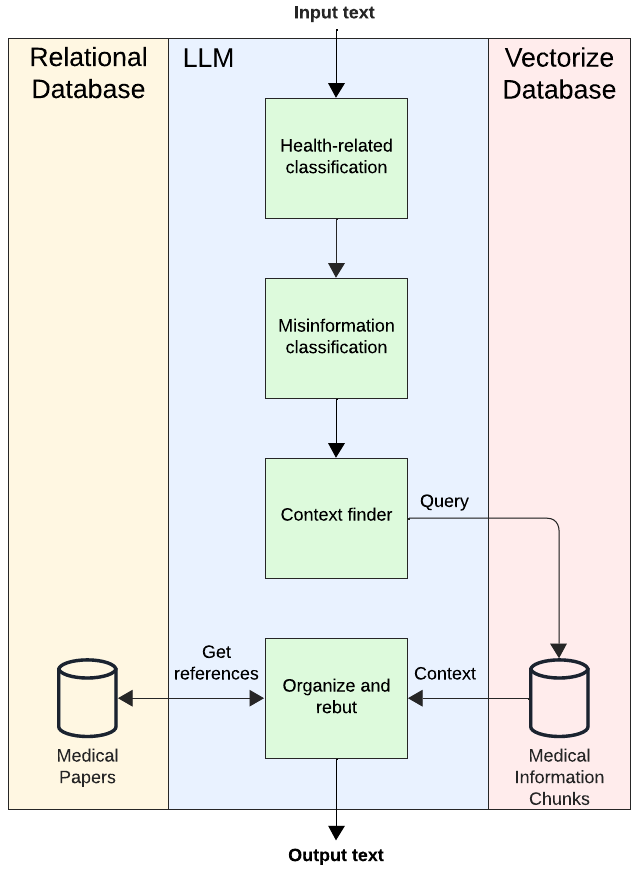
\includegraphics[width=0.75\textwidth]{images/LLM_Pipeline} %specify width
	\end{center}
	\caption{Misinformation Rebuttal LLM System Architecture} %specify caption
	\label{fig:llm}
\end{figure}

\section{Hardware and Software}
\list{-}
    \item V100 machines: 32Gb VRAM, and 80-ish RAM
    \item Cuda 11.7
    \item Python 3.9.19
    \item Pytorch 2.0.1
    \item Transformers 4.34.0

